\section{Logistic Regression}

    \subsection{Classification}
        
        \begin{itemize}
            \item Binary Classification: y $\in \{0, 1\}$, where 0 denotes the negative class; 1 denotes the positive class.
            \item Multi-class Classification:y $\in \{0, 1, \cdots, n\}$ 
        \end{itemize}

        We will be using binary classification: 
        \begin{itemize}
            \item Linear regression is not suitable for classification: since $h_\theta (x)$ can output out of range, i.e. <0 or >1. 
            \item We will use \textbf{logistic regression}, which ensures that the output $h_\theta (x)$ is between 0 and 1.
        \end{itemize}

    \subsection{Hypothesis Representation}

        \subsubsection{Logistic function}
            The idea is to have $ 0 \leq h_\theta (x) \leq 1$. Instead of the linear regression hypothesis: $h_\theta (x) = \theta^T x$, we will instead let:
                \[
                    h_\theta (x) = g (\theta^t x)
                ,\]

                where \[
                    g(z) = \frac{1}{1+e^{-z}}
                \]

                g(z) is known as the \textbf{logistic function}, also known as the Sigmoind function. Figure \ref{fig:sigmoid-function} shows a plot of the logitstic function, which ranges from 0 to 1. 


                which yields 
                \begin{equation}
                    h_\theta (x) = \frac{1}{1+e^{-z}}
                    \label{eq:log-reg-hypo}
                \end{equation}


                \begin{figure}[htbp]
                    \centering
                    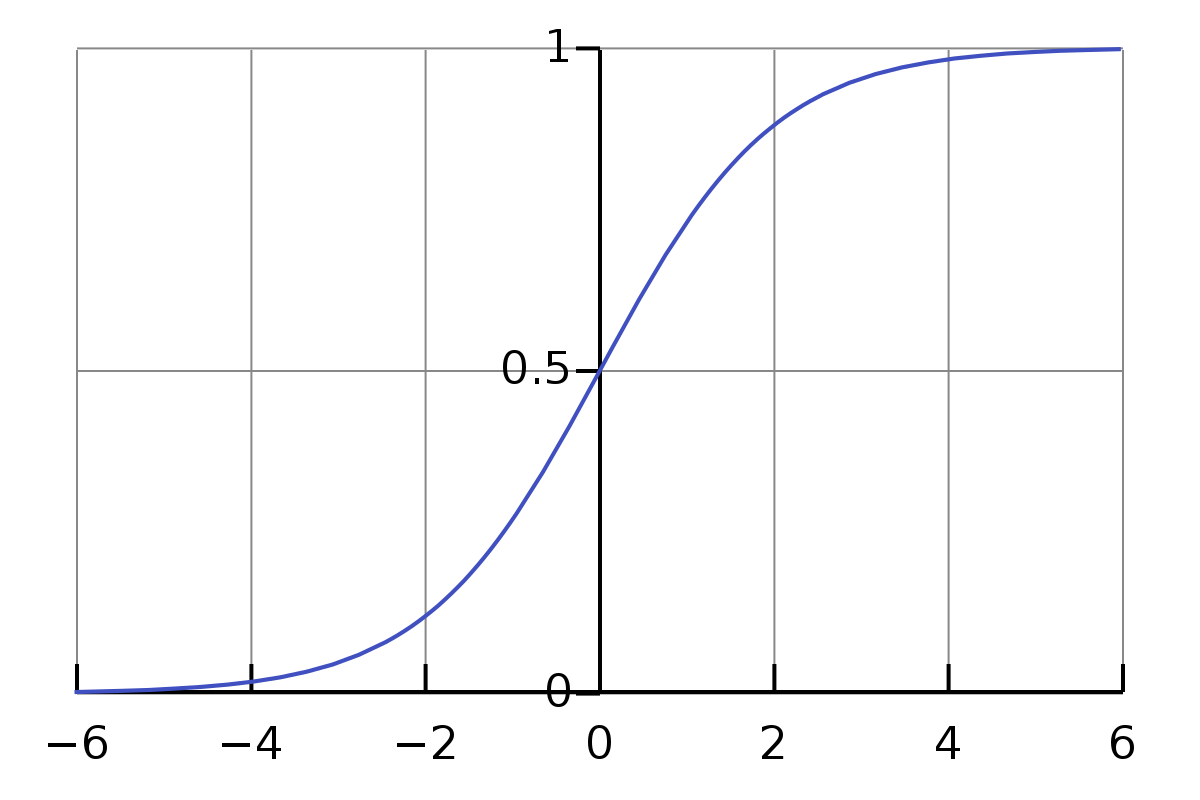
\includegraphics{'image/sigmoid-function.png'}
                    \caption{Sigmoid Function}
                    \label{fig:sigmoid-function}
                \end{figure}


        \subsubsection{Interpretation of Hypothesis Output}
        $ h_\theta (x)= $ estimated probability that y= 1 on input x. For example, $h_\theta(x)= 0.7$ gives us a probability of 70\% that are output is 1. 
        From a probability theory point of view, one can express $h_\theta (x)$ as $ P(y=1 \mid x;\theta)$. 

        Note that since this is a probability and the total probability sums up to 1, and the real y can only be either 0 or 1:
        \[
            P(y=0 \mid x; \theta) + P(y=1 \mid x;\theta) = 1
        \] 
            


    \subsection{Decision Boundary}

        Recall so far we have $h_\theta (x) = g(\theta^T) x$ and $g(z) = \frac{1}{1+exp(-z)}$. Suppose we set $h_\theta(x) = 0.5$ to be our determining factor for whether y= 0 or y =1. Note that from \ref{fig:sigmoid-function}, one can observe that $h_\theta(x) = 0.5$ corresponds to $\theta^T x = 0$, which is the \textbf{decision boundary}. The decision boundary is the equation which separates the different classes on a plot. There are linear and non-linear decision boundaries.


    \subsection{Cost function}

        Previously, we had $ J(\theta) = \frac{1}{m} \sum_{i=1}^{m} Cost( h_\theta ( x^{(i)}), y^{(i)} )$, where $Cost (h_\theta(x), y) = \frac{1}{2} (h_\theta(x) - y)^2$. 
        Now, the definition of the hypothesis $h_\theta$ has changed to $\frac{1}{1+exp(-\theta^T x}$, as a result the cost function is now non-convex. 
        
            \textbf{Logistic Regression Cost Function}

            Therefore, a new cost function definition is needed. We propose: 
            \[
                Cost(h_\theta(x), y) = 
                \begin{cases}
                    -log(h_\theta(x))       &\quad \text{if } y=1
                    -log(1- h_\theta(x))    &\quad \text{if } y=0
                \end{cases}
            \] 

            <INSERT FIGURE>
            Note that Cost=0, if y=1, $h_\theta(x) =1$; but as $h_\theta(x) \to 0$, then $Cost \to \infty$. This proposition captures the intuition that if $h_\theta(x)=0$, predict $P(y=1 \mid x;\theta)$, but y ends up being 1, we will penalize the learning algorithm by very large cost.
